% This section provides a high-level outline of the proposed system or solution. It typically illustrates the system architecture or the interactions between the different solution components (via a “boxes-and-arrows” diagram) from a user’s perspective.

\mytodo{intro chapter on Overall design}

A joint data-driven technique and machine learning algorithms approach are used in this work for this classification task. Before the classification step, number of new features are generated or engineered from the internal company data. the insight from the experts are considered first, then from the historical reports the data driven method was used to prepare a dataset to train the desired model. Based on statistical correlation the important features are selected as final features to train various Ensemble models and artificial neural networks are used to get the best out come. \mytodo{refer the the three step flow}

Firs step of data driven approach is to apply the theory of change. As per the theory of change we can find the road map for how to get company information which are most useful. This method also help to find how to archive long time goals along with indicator for improve and track progress. Then its important to get in touch with internal experts to understand what sort of data they are using for daily tasks.

Generally the classifiers perform quite weak due to missing values and imbalance dataset for real life scenarios. The one of the major reason for the missing data is the collected data does not contain enough information, because of he statistical error or some missing values. To obtain more hidden
information, data-driven method generally is a good choice. In the data driven approach hidden features can be found based on feedback from expert

Data-driven decision making means getting the right data to the right model to the right time to improve the model for problem solving. This approach can help the organisation to identify and apply recent trend in data to apply it for finding solutions.

\subsection{Proposed architect}\label{subsec:propsed-architech}
\mytodo{fill architect section}
\begin{figure}[ht]
    \centering
    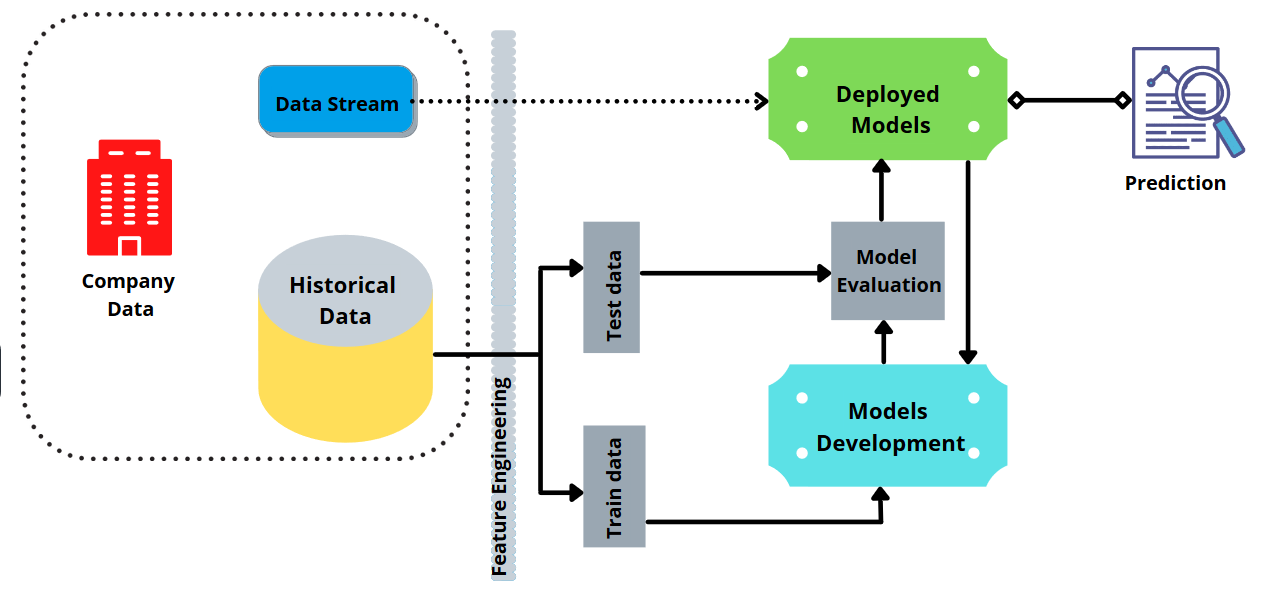
\includegraphics[width=\linewidth]{figures/overall_design.PNG}
    \caption{Overall Design}
    \label{fig:design}
\end{figure}

\mytodo{highlight the coverage in this paper}

\subsection{Imbalance Class Problem}\label{subsec:imbalance-class-problem}
Training classification model using imbalance data set generally leads to bias to predict one sample from another. Considering the fraudulent or suspicious number of companies are so less, the training data set for fraud detection is highly imbalanced. Before training the classifier, the data set can be fixed by using below sampling methods.    
\subsubsection{Under-sampling:}\hspace*{\fill} \\
Under sampling is one of the common and basic method of sampling to reduce class biases \cite{10.1145/3055635.3056643}. In this method a selective number of (generally equal number of smaller class data) samples are taken from large class. The samples are randomly taken and number of instances are based on minority class. This method provide the smaller dataset than the actual one as the number of instances for majority class reduces dramatically. 
\subsubsection{Over-sampling}\hspace*{\fill} \\
For over sampling method, the more samples are taken from the minority class so that the main dataset becomes balanced. Even though the random sampling method is used for taking samples, but due to class imbalance, we can see that number of repeated instances are copied from the minority class to prepare the dataset. This method provide the larger dataset as the number of instances for minority class increases. 

\subsubsection{SMOTE}\hspace*{\fill} \\
SMOTE is a synthetic over sampling method \cite{2002}. SMOTE drastically improve the performance of classifying minatory class by creating synthetic samples. Generally the synthetic samples are randomly generated by randomly selected minority class samples with interpolation between the neighbours of the selected sample. SMOTE facilitate balanced dataset with related minority class samples to learn from, which allows the models to decision boarder regions,  leading coverage of the minority class.

\subsubsection{Combined Sampling}\hspace*{\fill} \\
In the combined sampling method two or more samplings method are used in the same data set \cite{10.1145/3055635.3056643}. Under and over sampling is a common approach. In this method the under-sampling of majority class and over-sampling of minority class are done to prepare the Dataset. Another suitable method is to under-sample the majority class and synthetic sampling minority class. 

% Source from paper 31
\subsection{Model Selection}\label{subsec:model-selection}

\subsection{Ensemble learning}\label{subsec:ensemble-learning}\hspace*{\fill} \\
As they use a collection of results to make a final decision, they are referred to as ensemble techniques.
\mytodo{small about ensemble learning}

\begin{outline}
 \1 \textbf{Random Forests:} Random forest classified is designed based on decision tree A is a decision tree in classification tree which each node has a  decision based on binary whether  $x_i < \alpha$ or $\alpha$  not for a fixed. The random forests classifiers are a combination of large number of decision tree  algorithms \cite{breiman2001random} ensemble together. Random forest algorithm is designed in a such a way that it combines a large number of relatively uncorrelated decision tress \cite{breiman2001random}. The random forest performs better than a singe decision tree specially to handling over-fitting and under-fitting for the training set \cite{Mishra2021}. The performance of the random forest algorithm depends on the strength of the individual tress in the forest and the correlation between them. This algorithm also introduce feature randomness by picking up only from a random subset of features which allows it to perform better with classification without over-fitting the training data set. Random forest constructed many individual decision tress at training. Prediction from all trees are pooled to make the final prediction; the mode of the classes for classification.  
 
 \2 Feature Importance: Feature importance is defined based on the probability of finding that particular node. The probability is calculated by ratio of samples reach that node. The higher value gets more importance in feature space. 
 
 \2 Gini Impurity: Gini impurity is used for classification tasks. $\sum_{i=1}^{C} f_i{(1-f_i)}$, \textbf{$f_i$} is the frequency of label i at a node and \textbf{C} is the number of unique labels. 
 
 \2 Information gain: Information gain is used for splitting the data using entropy. This is calculated as the change in entropy after the dataset split on an attribute. $Gain(T,X) = Entropy(T) - Entropy(T,X)$, here \textbf{T} is target variable, \textbf{X} is the feature to be split on \textbf{Entropy(T,X)} which is calculated after the data is split on feature. \mytodo{cite}
 
 $$ni_j =w_jC_j - w_{left(j)}C_{left(j)} - w_{right(j)}C_{right(j)}$$
 

 %\cite https://towardsdatascience.com/the-mathematics-of-decision-trees-random-forest-and-feature-importance-in-scikit-learn-and-spark-f2861df67e3%
 
 \1 \textbf{XGBoost:} XGBoost is an ensemble method with the main goal of reducing bias and variance. Gradient boosting which employs the gradient descent algorithm to minimise loss \cite{Chen:2016:XST:2939672.2939785}. The algorithm forms trees sequentially and each new tree aims to reduce the error of the previous tree (10). The feature weights are readjusted and each new tree learns from its ancestors and the residual error is updated. A strong model is formed by combining successive weak learners which have high bias to make the final prediction thus reducing both bias and variance.
\end{outline}




\subsubsection{Neural Network}
\mytodo{briefing about neural network}
\tikzset{%
  every neuron/.style={
    circle,
    draw,
    minimum size=0.5cm
  },
  neuron missing/.style={
    draw=none, 
    scale=2,
    text height=0.333cm,
    execute at begin node=\color{black}$\vdots$
  },
}

\begin{figure}[h]
    \centering
        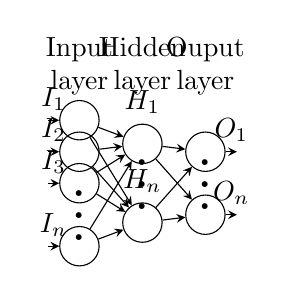
\begin{tikzpicture}[x=.4cm, y=0.4cm, >=stealth]
        
            \foreach \m/\l [count=\y] in {1,2,3,missing,4}
              \node [every neuron/.try, neuron \m/.try] (input-\m) at (0,2.5-\y) {};
            
            \foreach \m [count=\y] in {1,missing,2}
              \node [every neuron/.try, neuron \m/.try ] (hidden-\m) at (2,2-\y*1.25) {};
            
            \foreach \m [count=\y] in {1,missing,2}
              \node [every neuron/.try, neuron \m/.try ] (output-\m) at (4,1.5-\y) {};
            
            \foreach \l [count=\i] in {1,2,3,n}
              \draw [<-] (input-\i) -- ++(-1,0)
                node [above, midway] {$I_\l$};
            
            \foreach \l [count=\i] in {1,n}
              \node [above] at (hidden-\i.north) {$H_\l$};
            
            \foreach \l [count=\i] in {1,n}
              \draw [->] (output-\i) -- ++(1,0)
                node [above, midway] {$O_\l$};
            
            \foreach \i in {1,...,4}
              \foreach \j in {1,...,2}
                \draw [->] (input-\i) -- (hidden-\j);
            
            \foreach \i in {1,...,2}
              \foreach \j in {1,...,2}
                \draw [->] (hidden-\i) -- (output-\j);
            
            \foreach \l [count=\x from 0] in {Input, Hidden, Ouput}
              \node [align=center, above] at (\x*2,2) {\l \\ layer};
        
        \end{tikzpicture}
    \caption{Neural Network}
    \label{fig:neural network}
\end{figure}

\begin{outline}
 \1 Activation functions 
   \2 Sigmoid: label/multi-label binary classification. in equation \ref{eq:sigmoid}
   \2 relu: 
 \1 Loss Functions
    \2 Cross Entropy: In binary classification, where the number of classes \textbf{M} equals 2, Binary Cross-Entropy(BCE) can be calculated as shown in equation \ref{eq:Cross Entropy}. 
 \1 Optimiser
    \2 Adam: Adaptive Moment Estimation (Adam) [14] is another method that computes adaptive learning rates for each parameter. In addition to storing an exponentially decaying average of past squared gradients vt like Adadelta and RMSprop, Adam also keeps an exponentially decaying average of past gradients mt, similar to momentum. Whereas momentum can be seen as a ball running down a slope, Adam behaves like a heavy ball with friction, which thus prefers flat minima in the error surface $m_n = E[X^n]$, here $m$ is momentum and $X$ is a random variable. 
 \1 Regularisation
    \2 L1: A regression model that uses L1 regularisation technique is called Lasso Regression. \ref{eq:L1}
    \2 L2: A regression model that uses L2 regularisation technique is called Ridge Regression. \ref{eq:L2}

\end{outline}


\begin{equation} \label{eq:sigmoid}
    Sigmoid: \sigma(z) = \frac{1} {1 + e^{-z}}
\end{equation}

\begin{equation} \label{eq:Relu}
    Relu(z) = max(0, z)
\end{equation}


\begin{equation} \label{eq:Cross Entropy}
   Cross Entropy Loss: -{(y\log(p) + (1 - y)\log(1 - p))}
\end{equation}

\begin{equation} \label{eq:L1}
    L1: Loss = Error(Y - \widehat{Y}) + \lambda \sum_1^n |w_i|
\end{equation}

\begin{equation} \label{eq:L2}
    L2: Loss = Error(Y - \widehat{Y}) +  \lambda \sum_1^n w_i^{2}
\end{equation}

\subsection{Tools of Trade}\label{subsec:tools-of-trade}

\subsubsection{Receiver Operating Characteristic (ROC):}\hspace*{\fill} \\
Receiver operating characteristics (ROC) graphs are useful for organising classifiers and visualising their performance. ROC graphs are commonly used in medical decision making, and in recent years have been used increasingly in machine learning and data mining research. Although ROC graphs are apparently simple, there are some common misconceptions and pitfalls when using them in practice. The purpose of this article is to serve as an introduction to ROC graphs and as a guide for using them in research. \cite{FAWCETT2006861}

\subsubsection{Confusion Matrix:}\hspace*{\fill} \\
A confusion matrix is a tool to visualise the performance of the classifier in a matrix form \cite{Ting2017}. In a confusion matrix the true classes of the object and the prediction of the classifiers are presented in a two-dimensional matrix. For binary classification problem, confusion matrix is a widely used tool as it gives a clear view of the performance of the classifiers. 

\begin{equation} \label{eq:aqquracy}
    Accuracy = \frac{TP+TN}{TP+TN+FP+FN}
\end{equation}

\begin{equation} \label{eq:precision}
    Precision = \frac{TP}{TP+FP}
\end{equation}

\begin{equation} \label{eq:recall}
    Recall = \frac{TP}{TP+FN}
\end{equation}


\begin{table}[]

    \begin{tikzpicture}[
        box/.style={draw,rectangle,minimum size=2cm,text width=1.5cm,align=left}]
        \matrix (conmat) [row sep=.1cm,column sep=.1cm] {
        \node (tpos) [box,
            label=left:\( \mathbf{p'} \),
            label=above:\( \mathbf{p} \),
            ] {True \\ positive};
        &
        \node (fneg) [box,
            label=above:\textbf{n},
            label=above right:\textbf{total},
            label=right:\( \mathrm{P}' \)] {False \\ negative};
        \\
        \node (fpos) [box,
            label=left:\( \mathbf{n'} \),
            label=below left:\textbf{total},
            label=below:P] {False \\ positive};
        &
        \node (tneg) [box,
            label=right:\( \mathrm{N}' \),
            label=below:N] {True \\ negative};
        \\
        };
        \node [left=.05cm of conmat,text width=1.5cm,align=right] {\textbf{actual \\ value}};
        \node [above=.05cm of conmat] {\textbf{prediction outcome}};
    \end{tikzpicture}

    
    \caption{Confusion Matrix}
    \label{tab:Confusion Matrix}
\end{table}
\mytodo{fix the matrix}




\subsubsection{AUC Performance:}\hspace*{\fill} \\
in case of imbalanced dataset, only accuracy as metric is not suitable. As even a naive model will provide more than satisfactory results. Then tool like AUC is very useful, because AUC considers the classification performance by using both positive and negative example. Hence by using this method we can still able to find a reasonable model that classifies imbalanced classes. AUC can be generated by True positive rate (TPR) and false positive rate using the confusion matrix. 



\begin{equation} \label{eq:Sensitivity}
    Sensitivity = Recall = \frac{TP}{TP+FN}
\end{equation}

\begin{equation} \label{eq: Specificity}
    Specificity = \frac{TN}{FP+TN}
\end{equation}

AUC is calculated as the Area Under the \textbf{Sensitivity` (TPR)- (1-Specificity)(FPR)} Curve.


\subsection{Used Technologies}\label{subsec:used-technologies}
\mytodo{describe the used libraries  and table}